\section{Baseline Escarpment Phenology and Optical Artifact Controls}
\label{sec:baseline_brdf}

Internal round-1 exploratory scripts over the Sewanee Domain initially yielded elevational green-up lapses of 4.10--4.27~d/100~m---steeper than \citet{hopkins1918}'s 3.28~d/100~m rule---and an apparent $-1.72$~d/decade spring advance in unharmonized 1984--2024 Landsat records. Auditing those internal sensitivity runs isolates the exact source of both discrepancies (\cref{fig:hopkins_decomp}, \cref{tab:baseline_optical}).

A three-factor decomposition on 2001--2023 \texttt{MODIS MCD12Q2 v061} across the Sewanee region (holding 3DEP elevation and the DOY~45--180 window fixed, starting from $3.98$ vs.\ $4.09$~d/100~m in the legacy SRTM run) shows why the lapse rate shifts from $3.98$ to $3.19$~d/100~m. Starting from the 15\% onset band (\texttt{Greenup\_1}) with a Hansen $>50\%$ tree-cover mask and no QA filter yields $3.98 \pm 0.24$~d/100~m (SE; SD $= 1.17$, $n=23$~yr). Adding \texttt{QA\_Overall\_1} $\le 1$ changes the mean by $0.00$~d/100~m, and replacing Hansen tree cover with \texttt{NLCD-41} deciduous forest shifts it by only $+0.01$~d/100~m (to $3.98 \pm 0.24$~d/100~m SE; SD $= 1.16$). Virtually the entire shift ($-0.80$~d/100~m) comes from switching to the 50\% half-amplitude band (\texttt{MidGreenup\_1}, matching Sentinel-2 \texttt{SOS50}), which averages $3.19 \pm 0.17$~d/100~m (SE; SD $= 0.82$), within 3\% of Hopkins' 3.28~d/100~m benchmark (\cref{fig:hopkins_decomp}b). Early 15\% onset and 50\% mid-greenup measure distinct phenophases that can legitimately lapse at different rates; using the matched 50\% definition reconciles MODIS with Hopkins' rule. Over 2001--2023, neither \texttt{MidGreenup\_1} timing ($-0.38 \pm 1.72$~d/decade SE, $p=0.83$) nor the elevational lapse ($-0.05 \pm 0.26$~d/100~m/decade SE, $p=0.86$) trends significantly, though interannual spring timing responds strongly to March--April temperature ($-2.40 \pm 0.65$~d/$^\circ$C SE, $r=-0.63$, $p=0.0014$).

In the unharmonized 1984--2024 Landsat Collection~2 record, adding a binary indicator for the 2013 Landsat~8 OLI atmospheric-processor transition (\texttt{LEDAPS} to \texttt{LaSRC}) exposes collinearity non-identifiability ($r=0.80$, $\text{VIF}=2.7$): neither the 2013 step ($-0.42 \pm 3.69$~d SE, $p=0.91$) nor the linear trend ($-1.58 \pm 1.46$~d/decade SE, $p=0.29$) can be separated reliably without cross-sensor radiometric harmonization. Over the longer century scale, raw \texttt{NOAA GHCN-Daily} records at Sewanee (\texttt{USC00408184}, 1895--1943 vs.\ 2000--2025, across a 1944--1999 temperature hiatus) show $+0.83^\circ$C warmer March--April mean temperature (Welch $p=0.029$), $-7.5$~d earlier last spring freeze ($p=0.036$), $+10.1$~d longer frost-free season ($p=0.021$; \cref{fig:hopkins_decomp}c), and flat autumn mean temperature ($+0.00^\circ$C, $p=0.995$). Because raw GHCN-Daily data are unadjusted for time-of-observation bias, instrument changes, or station micro-moves across the 56-year hiatus, these shifts provide contextual background rather than homogenized climate attribution.

\begin{table}[t]
\centering
\begin{threeparttable}
\caption{\textbf{MODIS three-factor baseline decomposition, optical/BRDF controls, and LAL harvest checks.} Every $\pm$ interval explicitly indicates SE or SD.}
\label{tab:baseline_optical}
\footnotesize
\begin{tabularx}{\linewidth}{@{} >{\raggedright\arraybackslash}p{0.42\linewidth} r r >{\raggedright\arraybackslash}X @{}}
\toprule
Diagnostic Test & Primary Estimate & Uncertainty / Metric & Interpretation \\
\midrule
\multicolumn{4}{@{}l}{\textit{Part A: MODIS 3-Factor Decomposition (2001--2023, $n=23$~yr) and Station Context}} \\
MODIS \texttt{Greenup\_1} (15\%, Hansen $>50\%$, no QA) & $3.98$~d/100~m & $\pm 0.24$ SE ($1.17$ SD) & Steeper early-onset lapse \\
MODIS \texttt{Greenup\_1} (15\%, \texttt{NLCD-41}, $\text{QA}\le 1$) & $3.98$~d/100~m & $\Delta=+0.01$ vs.\ above & QA/conifer effect negligible \\
MODIS \texttt{MidGreenup\_1} (50\%, \texttt{NLCD-41}, $\text{QA}\le 1$) & $3.19$~d/100~m & $\pm 0.17$ SE ($0.82$ SD) & Matches Hopkins (3.28); trend $p=0.86$ \\
MODIS sensitivity (Mar--Apr $T_{\text{mean}}$) & $-2.40$~d/$^\circ$C & $\pm 0.65$ SE, $p=0.0014$ & Strong interannual coupling \\
Raw NOAA Mar--Apr shift (2000--25 vs.\ 1895--43)$^\dagger$ & $+0.83^\circ$C & Welch $p=0.029$ & Unhomogenized station context \\
\midrule
\multicolumn{4}{@{}l}{\textit{Part B: Optical / BRDF Invariance (2018--2024, $n=7$~yr) and LAL Harvest Controls}} \\
Signal~A: Raw S2 NDRE ($\Delta$SOS / $\Delta$EOS) & $+3.86$ / $-2.98$~d & $\pm 0.50$ / $\pm 1.36$ SE & Uncorrected baseline \\
Signal~A: \texttt{SCS+C} S2 NDRE ($\Delta$SOS / $\Delta$EOS) & $+3.84$ / $-2.92$~d & 99.6\% / 98.1\% ret. & Illumination-invariant \\
Signal~A: BRDF-norm \texttt{HLS v2.0} NDRE & $+3.10$ / $-2.45$~d & NDVI $+3.33$ / $-2.19$~d & Cross-sensor replicated \\
Signal~A: Excl.\ all 120 LAL harvests ($N=1$ cove) & $+5.28$~d (SOS) & $n=42/13$ px (descr.) & Descriptive single-cove check \\
Signal~B: \texttt{SCS+C} NDRE (N/E/S/W) & $+2.30$ to $+2.61$~d & HLS $+2.77$ to $+3.32$~d & Aspect-invariant \\
Signal~B: Excl.\ all 120 LAL harvests ($n=435$~px) & $+2.62$~d (SOS) & 2~km block $p \le 0.0032$ & Survives unlogged stands \\
\bottomrule
\end{tabularx}
\begin{tablenotes}[flushleft]
\footnotesize
\item $^\dagger$Raw GHCN-Daily \texttt{USC00408184}; unadjusted for TOBS, instrument transitions, or 1944--1999 hiatus. Internal gate P2 status: \texttt{PARTIAL\_OR\_FAIL}.
\end{tablenotes}
\end{threeparttable}
\end{table}

\subsection{Optical/BRDF Invariance and Internal-Criterion Vertical Decoupling Null}
Applying \texttt{SCS+C} topographic illumination correction to Sentinel-2 preserves 99.6\% of Lost Cove's spring delay ($+3.84$~d) and 98.1\% of its autumn advance ($-2.92$~d) in red-edge NDRE (\cref{fig:brdf_decoupling}a). BRDF-normalized NASA \texttt{HLS v2.0} reproduces both signs ($+3.10$~d SOS and $-2.45$~d EOS in NDRE; $+3.33$~d and $-2.19$~d in NDVI), and inside mesophytic cove forest (\texttt{EVT 3321}), \texttt{SCS+C} NDRE ($+3.02$, $-5.31$~d) closely tracks \texttt{HLS v2.0} NDRE ($+3.03$, $-5.30$~d). On the plateau cap, Signal~B remains uniform across all four cardinal aspect quadrants ($+2.61$~d North, $+2.37$~d East, $+2.30$~d South, and $+2.56$~d West in \texttt{SCS+C} NDRE; \cref{fig:brdf_decoupling}b), ruling out solar-geometry or BRDF artifacts. Masking all 120 public Sewanee Landscape Analysis Lab timber-harvest polygons leaves Lost Cove's descriptive single-cove spring contrast at $+5.28$~d ($n=42$ Lost Cove vs.\ $13$ OpenN pixels; pixel-level $p$-values are omitted for $N=1$ cove due to spatial pseudoreplication) and leaves Signal~B intact at $+2.62$~d across all 25 spatial block-grid origins ($1$~km $p \le 0.00063$; $2$~km $p \le 0.0032$, \cref{tab:baseline_optical}).

Under internal decision criterion P2, we also tested whether late-April radiative freezes widen the gap between understory-sensitive NDVI and crown-sensitive NDRE ($\Delta\text{SOS}_{\text{NDVI}} - \Delta\text{SOS}_{\text{NDRE}}$) in Lost Cove. Across the seven Sentinel-2 years (2018--2024), this criterion failed ($r=-0.20, p=0.66$; freeze vs.\ mild springs $p=0.76$; \cref{fig:brdf_decoupling}c), yielding an overall P2 internal status of \texttt{PARTIAL\_OR\_FAIL}. The 2019 minimum ($-2.2^\circ$C on April~1, DOY~91, prior to budbreak) produced negative decoupling ($-2.36$~d). Although \texttt{HLS v2.0} correlated with April minimum temperature ($r=-0.79, p=0.036$) and an exploratory post-DOY-100 frost split separated Sentinel-2 years ($+1.70$ vs.\ $-0.84$~d, $p=0.025$), vertical decoupling remains unconfirmed.

\begin{figure}[t]
\centering
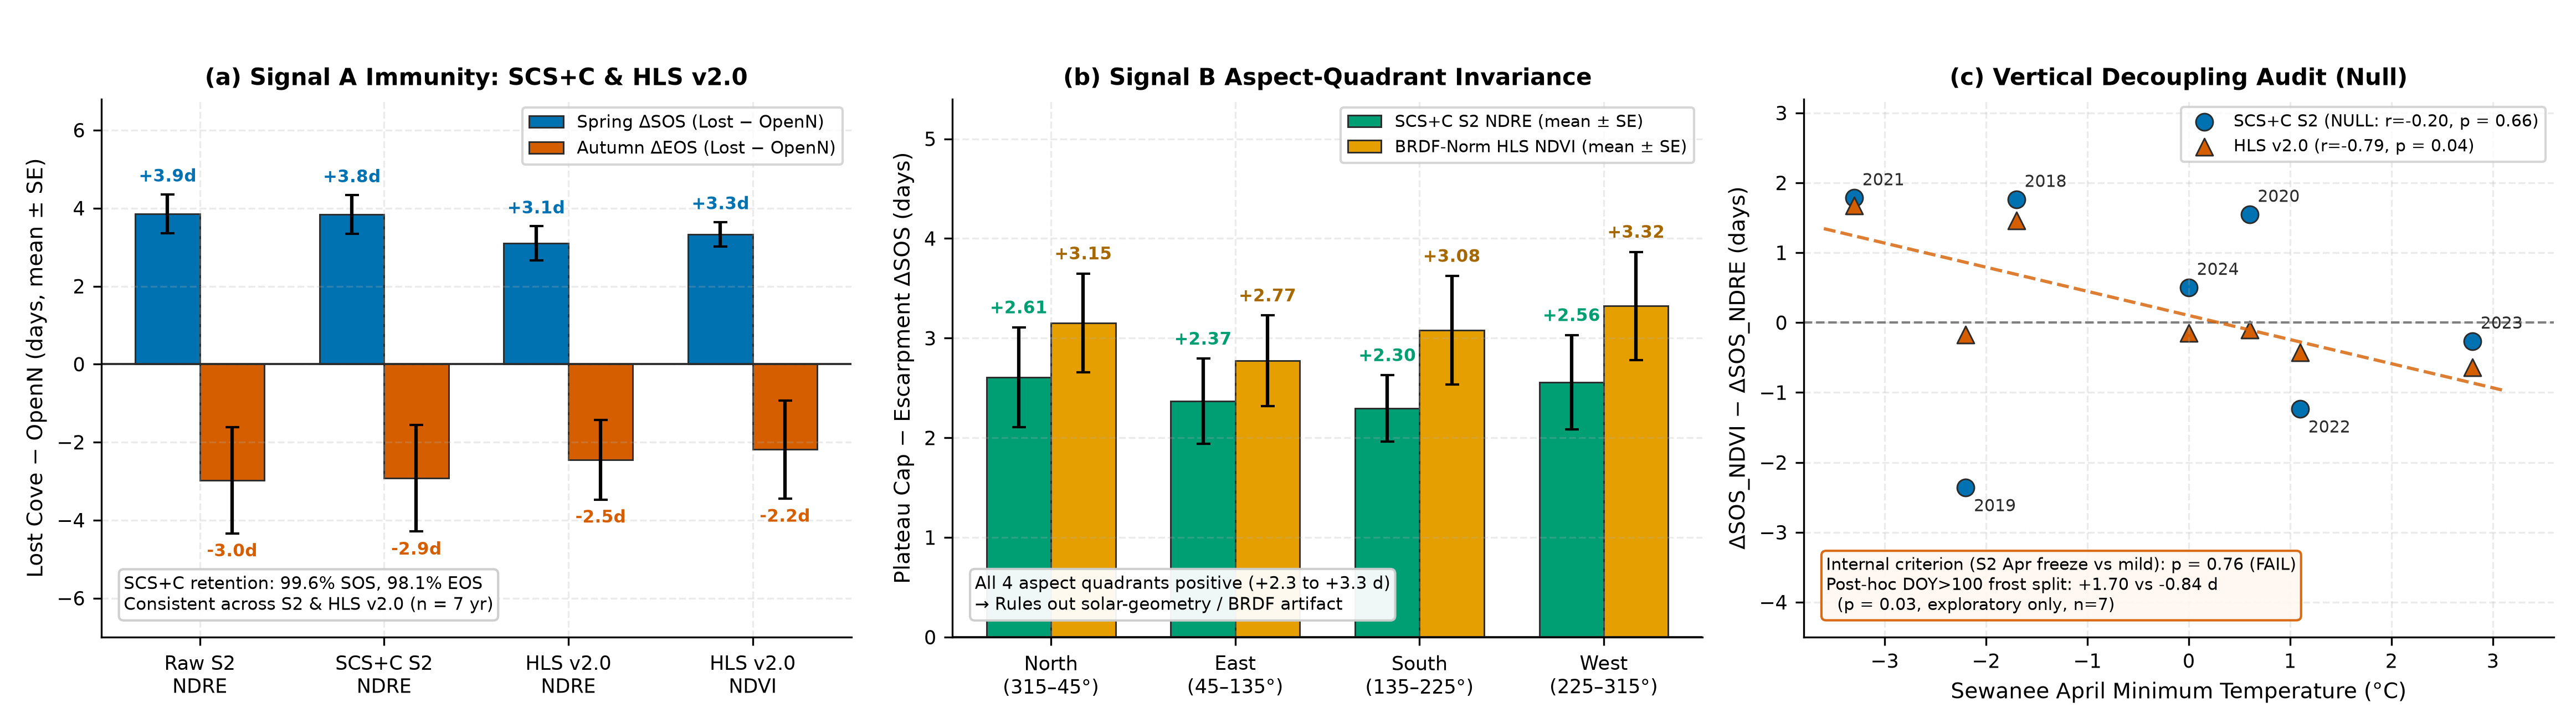
\includegraphics[width=\linewidth]{figures/fig2.png}
\caption{\textbf{Both phenological anomalies survive topographic and BRDF correction, whereas the internal vertical-decoupling test fails.} (a)~Lost Cove minus Open North Cove shifts (mean $\pm$ SE, $n=7$~yr) remain stable across raw Sentinel-2, \texttt{SCS+C} Sentinel-2, and BRDF-normalized NASA \texttt{HLS v2.0}. (b)~Plateau-cap spring delay (Signal~B, mean $\pm$ SE) holds across all four cardinal aspect quadrants, ruling out solar-geometry bias. (c)~Sentinel-2 vertical decoupling ($\Delta\text{SOS}_{\text{NDVI}} - \Delta\text{SOS}_{\text{NDRE}}$) shows no relation to April minimum temperature ($r=-0.20, p=0.66$).}
\label{fig:brdf_decoupling}
\end{figure}
